\documentclass[10pt]{article}
\usepackage[a4paper,left=17mm,right=17mm,top=15mm,bottom=16mm,headheight=12pt,footskip=8mm]{geometry}
\usepackage{lmodern}
\usepackage{fontspec}
\setmainfont{Arial}
\setsansfont{Arial}
\setmonofont{Consolas}
\usepackage{amsmath,amssymb}
\usepackage{xcolor}
\definecolor{Navy}{HTML}{18324B}
\definecolor{Teal}{HTML}{177F82}
\definecolor{Blue}{HTML}{547B9A}
\definecolor{Ink}{HTML}{263B4A}
\definecolor{Muted}{HTML}{536B7A}
\definecolor{Rule}{HTML}{D9E3E9}
\definecolor{Pale}{HTML}{F3F7F9}
\definecolor{TealPale}{HTML}{EDF6F5}
\definecolor{Warm}{HTML}{AE613F}
\definecolor{WarmPale}{HTML}{FCF2EC}
\usepackage{tikz}
\usetikzlibrary{arrows.meta,positioning,calc,fit,backgrounds}
\usepackage{pgfplots}
\pgfplotsset{compat=1.18}
\usepackage{fancyhdr}
\usepackage{hyperref}
\hypersetup{colorlinks=true,urlcolor=Teal,linkcolor=Teal,
  pdftitle={Correct Outputs, Contaminated Search: Independent Research Highlight},
  pdfauthor={Zhijing Wu},
  pdfsubject={Independent research technical note on branch isolation in executable world models},
  pdfkeywords={world models, agent planning, executable simulation, branch isolation, WCTR},
  pdflang={en-US},pdfdisplaydoctitle=true}
\pagestyle{fancy}
\fancyhf{}
\renewcommand{\headrulewidth}{0pt}
\renewcommand{\footrulewidth}{0.4pt}
\renewcommand{\footrule}{\hbox to\headwidth{\color{Rule}\leaders\hrule height\footrulewidth\hfill}}
\fancyfoot[L]{\fontsize{9.2}{11}\selectfont\color{Muted}Zhijing Wu\quad/\quad Sichuan University\quad/\quad October 2026}
\fancyfoot[R]{\fontsize{9.2}{11}\selectfont\color{Navy}\thepage\ / 2}
\setlength{\parindent}{0pt}
\setlength{\parskip}{4.2pt}
\setlength{\fboxsep}{8pt}
\color{Ink}
\fontsize{10.4}{13.8}\selectfont
\newcommand{\bodyfont}{\fontsize{10.4}{13.8}\selectfont}
\newcommand{\smallnote}{\fontsize{9.2}{12}\selectfont\color{Muted}}
\newcommand{\eyebrow}[1]{{\fontsize{9.4}{12}\selectfont\bfseries\color{Teal}#1}\par}
\newcommand{\sectionline}[2]{\par\vspace{6pt}{\fontsize{13}{16}\selectfont\bfseries\color{Navy}{\color{Teal}#1}\enspace #2}\par\vspace{3pt}}
\newcommand{\figcaption}[2]{{\smallnote\textbf{\color{Navy}#1}\enspace #2\par}}
\tikzset{
  flow/.style={-{Stealth[length=2.1mm,width=1.5mm]},line width=.8pt,draw=Muted},
  warmflow/.style={flow,draw=Warm},
  tealflow/.style={flow,draw=Teal},
  box/.style={rounded corners=2pt,draw=Rule,fill=white,line width=.7pt,
    minimum height=10mm,text width=21mm,align=center,inner sep=3pt,font=\fontsize{9.3}{11.5}\selectfont},
  smallbox/.style={rounded corners=2pt,draw=Rule,fill=white,line width=.7pt,
    minimum height=13mm,text width=27mm,align=center,inner sep=3pt,font=\fontsize{9.3}{11.5}\selectfont}
}

\newcommand{\protocolitem}[2]{\noindent
  \makebox[6mm][l]{\color{Teal}\bfseries #1}%
  \begin{minipage}[t]{\dimexpr\linewidth-6mm\relax}#2\end{minipage}\par\vspace{4pt}}
\begin{document}
\bodyfont
\eyebrow{INDEPENDENT RESEARCH TECHNICAL NOTE}
\vspace{4pt}
{\fontsize{25}{28}\selectfont\bfseries\color{Navy}
Correct outputs,\\contaminated search\par}
\vspace{5pt}
{\fontsize{12}{15}\selectfont\color{Muted}
A state-ownership contract for executable world models\par}
\vspace{6pt}
{\fontsize{10.7}{14}\selectfont
\textbf{Zhijing Wu}\quad\textcolor{Muted}{Sichuan University}\hfill
\href{https://zhijingwu.github.io/}{zhijingwu.github.io}\par}
\vspace{5pt}
{\color{Rule}\rule{\linewidth}{.7pt}}\par
\vspace{3pt}
{\fontsize{13.1}{17}\selectfont\bfseries\color{Navy}
Can a planner trust a model call that changes\\
the parent state of its hypothetical branches?\par}
\vspace{2pt}
I identified a state-ownership failure in released executable world models:
a call can return the same state values as a full-copy reference while
modifying nested objects owned by its caller. Sibling branches then start
from different parents, making search sensitive to rollout order.

\vspace{3pt}
% Original vector schematic. Values illustrate ownership, not a new experiment.
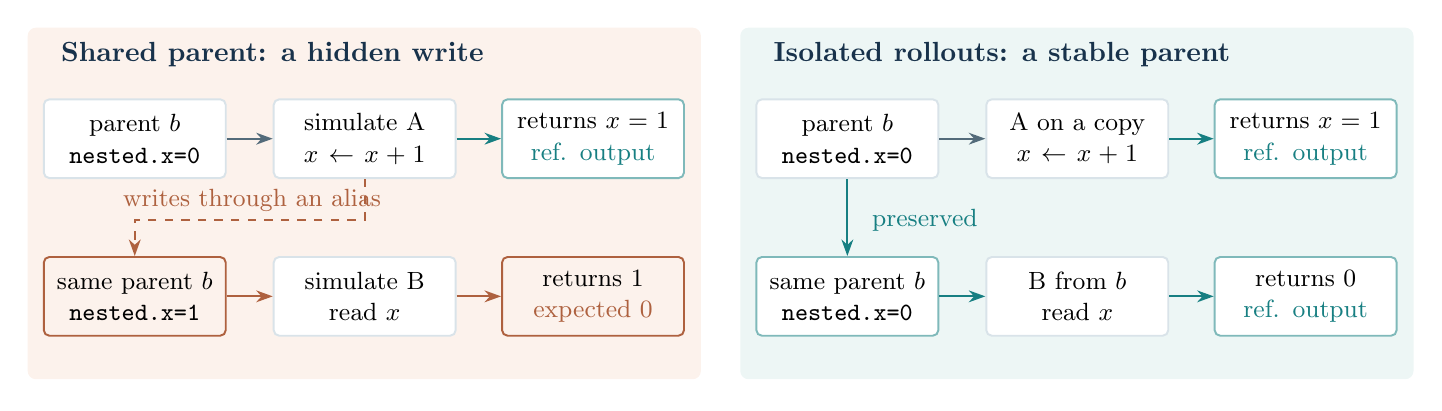
\begin{tikzpicture}[x=1cm,y=.94cm]
  \path[use as bounding box] (0,0) rectangle (17.6,4.8);
  \fill[WarmPale,rounded corners=3pt] (0,.05) rectangle (8.55,4.8);
  \fill[TealPale,rounded corners=3pt] (9.05,.05) rectangle (17.6,4.8);
  \node[anchor=west,font=\fontsize{10.2}{12}\selectfont\bfseries,text=Navy] at (.3,4.43) {Shared parent: a hidden write};
  \node[anchor=west,font=\fontsize{10.2}{12}\selectfont\bfseries,text=Navy] at (9.35,4.43) {Isolated rollouts: a stable parent};
  \node[box] (p) at (1.36,3.3) {parent $b$\\\texttt{nested.x=0}};
  \node[box] (a) at (4.28,3.3) {simulate A\\$x\leftarrow x+1$};
  \node[box,draw=Teal!55] (oa) at (7.18,3.3) {returns $x=1$\\\textcolor{Teal}{ref. output}};
  \draw[flow] (p.east)--(a.west);
  \draw[tealflow] (a.east)--(oa.west);
  \node[box,draw=Warm,fill=WarmPale] (badp) at (1.36,1.17) {same parent $b$\\\texttt{nested.x=1}};
  \node[box] (b) at (4.28,1.17) {simulate B\\read $x$};
  \node[box,draw=Warm,fill=WarmPale] (ob) at (7.18,1.17) {returns $1$\\\textcolor{Warm}{expected $0$}};
  \draw[warmflow,dashed] (a.south)--++(0,-.55)-|(badp.north);
  \node[font=\fontsize{9.2}{11}\selectfont,text=Warm] at (2.85,2.47) {writes through an alias};
  \draw[warmflow] (badp.east)--(b.west);
  \draw[warmflow] (b.east)--(ob.west);
  \begin{scope}[xshift=9.05cm]
    \node[box] (ip) at (1.36,3.3) {parent $b$\\\texttt{nested.x=0}};
    \node[box] (ia) at (4.28,3.3) {A on a copy\\$x\leftarrow x+1$};
    \node[box,draw=Teal!55] (ioa) at (7.18,3.3) {returns $x=1$\\\textcolor{Teal}{ref. output}};
    \draw[flow] (ip.east)--(ia.west);
    \draw[tealflow] (ia.east)--(ioa.west);
    \node[box,draw=Teal!55] (goodp) at (1.36,1.17) {same parent $b$\\\texttt{nested.x=0}};
    \node[box] (ib) at (4.28,1.17) {B from $b$\\read $x$};
    \node[box,draw=Teal!55] (iob) at (7.18,1.17) {returns $0$\\\textcolor{Teal}{ref. output}};
    \draw[tealflow] (ip.south)--(goodp.north);
    \node[anchor=west,font=\fontsize{9.2}{11}\selectfont,text=Teal] at (1.55,2.2) {preserved};
    \draw[tealflow] (goodp.east)--(ib.west);
    \draw[tealflow] (ib.east)--(iob.west);
  \end{scope}
\end{tikzpicture}
\par
\figcaption{Figure 1.}{Illustrative deterministic program. Action A's return matches
the full-copy reference in both panels; only the isolated parent remains reusable by B.}

\sectionline{01}{The mechanism I implemented: WCTR}
I implemented \textbf{Witness-Compiled Transactional Rollouts} to learn mutation
paths from executions, selectively fork their alias ancestors, and mark new
allocations private. Unexpected writes are journaled; output grafting preserves
the returned successor before parent rollback.\par
\vspace{2pt}
% Original vector mechanism diagram; exact implementation remains in Stage 2.
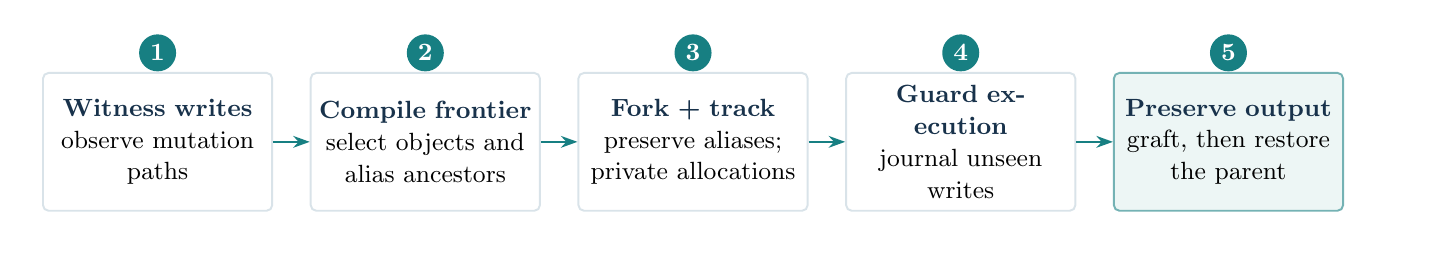
\begin{tikzpicture}[x=1cm,y=1cm]
  \path[use as bounding box] (0,0) rectangle (17.6,2.5);
  \foreach \x/\n in {1.65/1,5.05/2,8.45/3,11.85/4,15.25/5}{
    \node[circle,fill=Teal,text=white,minimum size=4.7mm,inner sep=0pt,
      font=\fontsize{9.3}{11}\selectfont\bfseries] at (\x,2.18) {\n};
  }
  \node[smallbox,minimum height=17.5mm] (w) at (1.65,1.05)
    {\textbf{\color{Navy}Witness writes}\\observe mutation\\paths};
  \node[smallbox,minimum height=17.5mm] (f) at (5.05,1.05)
    {\textbf{\color{Navy}Compile frontier}\\select objects and\\alias ancestors};
  \node[smallbox,minimum height=17.5mm] (fork) at (8.45,1.05)
    {\textbf{\color{Navy}Fork + track}\\preserve aliases;\\private allocations};
  \node[smallbox,minimum height=17.5mm] (g) at (11.85,1.05)
    {\textbf{\color{Navy}Guard execution}\\journal unseen\\writes};
  \node[smallbox,minimum height=17.5mm,draw=Teal!60,fill=TealPale] (r) at (15.25,1.05)
    {\textbf{\color{Navy}Preserve output}\\graft, then restore\\the parent};
  \draw[tealflow] (w.east)--(f.west);
  \draw[tealflow] (f.east)--(fork.west);
  \draw[tealflow] (fork.east)--(g.west);
  \draw[tealflow] (g.east)--(r.west);
\end{tikzpicture}
\par
\figcaption{Figure 2.}{Witnesses guide selective copying; runtime guards handle
unseen writes. Alias preservation and allocation tracking are part of the implementation.}

\vspace{5pt}
\colorbox{TealPale}{\begin{minipage}{\dimexpr\linewidth-2\fboxsep\relax}
  \centering
  {\fontsize{10}{13}\selectfont\bfseries\color{Navy}Operational target: an unchanged parent and full-copy-equivalent values\par}
  \vspace{4pt}
  $\displaystyle b_{\mathrm{after}}\equiv b_{\mathrm{before}},
  \qquad b'_a\equiv F\!\left(\operatorname{deepcopy}(b),a\right).$
\end{minipage}}\par
\vspace{3pt}
Equivalence is with the \textbf{same program}, not ground-truth prediction.
Checks cover instrumented dict, list, set and tuple operations; they establish
neither arbitrary-Python isolation nor theoretical novelty.

\vspace{5pt}
\colorbox{Pale}{\begin{minipage}{\dimexpr\linewidth-2\fboxsep\relax}
  \begin{minipage}[t]{.46\linewidth}
    {\fontsize{19}{22}\selectfont\bfseries\color{Teal}59 / 3,942\par}
    {\fontsize{10.2}{13}\selectfont\textbf{Discovery in BabyAI}\par}
    {\fontsize{10}{13}\selectfont input mutations in recorded predictions\par}
  \end{minipage}\hfill
  \begin{minipage}[t]{.51\linewidth}
    {\fontsize{19}{22}\selectfont\bfseries\color{Navy}0 / 33,692\par}
    {\fontsize{10.2}{13}\selectfont\textbf{Checked WCTR transitions}\par}
    {\fontsize{10}{13}\selectfont parent/output mismatches in the frozen live study\par}
  \end{minipage}\par
  \vspace{4pt}
  {\fontsize{9.6}{12.5}\selectfont\color{Muted}
  Finite workload checks; other protected controls also had zero parent/output mismatches.\par}
\end{minipage}}\par

\newpage
\eyebrow{SELECTED EVIDENCE / PROPOSED RESEARCH DIRECTION}
\vspace{4pt}
{\fontsize{22}{26}\selectfont\bfseries\color{Navy}
From branch isolation to decision trust\par}
\vspace{4pt}
I used controlled comparisons to separate an implementation's branch behavior,
bounded planning performance, and actual interactive task completion.

\sectionline{02}{A controlled planning result, with its boundary}
% Selected frozen result. Internal program-goal completion, not native success.
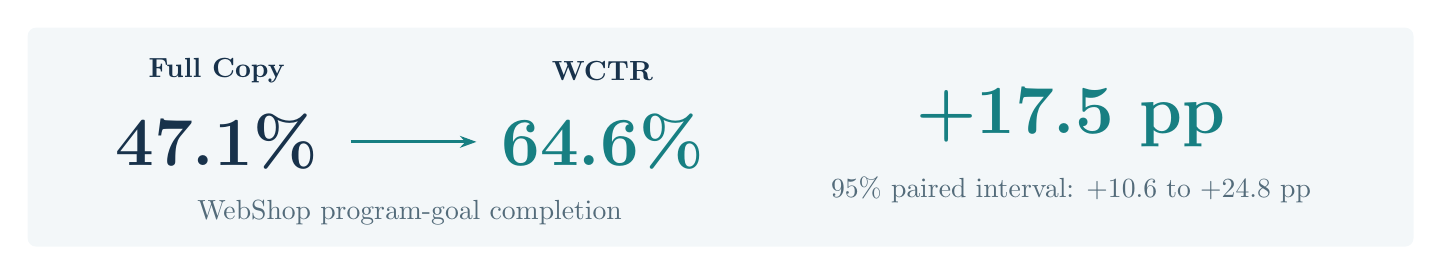
\begin{tikzpicture}[x=1cm,y=1cm]
  \path[use as bounding box] (0,0) rectangle (17.6,2.8);
  \fill[Pale,rounded corners=3pt] (0,.02) rectangle (17.6,2.8);
  \node[font=\fontsize{10.3}{13}\selectfont\bfseries,text=Navy] at (2.4,2.25) {Full Copy};
  \node[font=\fontsize{23}{26}\selectfont\bfseries,text=Navy] at (2.4,1.35) {47.1\%};
  \draw[tealflow,line width=1.1pt] (4.1,1.35)--(5.7,1.35);
  \node[font=\fontsize{10.3}{13}\selectfont\bfseries,text=Navy] at (7.3,2.25) {WCTR};
  \node[font=\fontsize{23}{26}\selectfont\bfseries,text=Teal] at (7.3,1.35) {64.6\%};
  \node[font=\fontsize{23}{26}\selectfont\bfseries,text=Teal] at (13.25,1.65) {+17.5 pp};
  \node[font=\fontsize{9.6}{12}\selectfont,text=Muted] at (13.25,.74) {95\% paired interval: +10.6 to +24.8 pp};
  \node[font=\fontsize{9.6}{12}\selectfont,text=Muted] at (4.85,.45) {WebShop program-goal completion};
\end{tikzpicture}
\par
{\fontsize{10}{13.2}\selectfont
\textbf{\color{Navy}Exact setting.} 80 generated structured-state goals, three timing
repeats, shared BFS (depth at most six; at most 4,096 expansions), and a
\textbf{soft 10\,ms planning deadline excluding setup and calibration}.
Completion was checked by independent full-copy execution of the released
program. The interval resamples source items in the frozen paired analysis.\par}
\vspace{3pt}
This is \textbf{not an improvement in native WebShop success}.
Controlled outcomes were mixed: Wordle declined from 54.2\% to 45.0\%
(\textcolor{Warm}{\textbf{-9.2 pp}}) under the same protocol.

\vspace{5pt}
\colorbox{Pale}{\begin{minipage}{\dimexpr\linewidth-2\fboxsep\relax}
  \textbf{\color{Navy}Native-task takeaway.}
  Full Copy, Top-Field, Journal Only and WCTR all completed
  \textbf{6/12 WebShop goals} and \textbf{43/100 Wordle seed tasks}.
  There was no incremental live-success benefit. With lifetime setup,
  verification and profiling charged, simpler protected controls were cheaper overall on
  this host; no general efficiency or superiority claim follows.\par
  \vspace{3pt}
  {\fontsize{9.6}{12.5}\selectfont\color{Muted}
  Native scope: small 1k-product WebShop catalog; released 40-word stochastic
  Wordle. The complete frozen archive remains authoritative.\par}
\end{minipage}}\par

\sectionline{03}{A small next experiment}
{\fontsize{16.1}{20}\selectfont\bfseries\color{Navy}
Which simulator errors can change the action a planner chooses?\par}
\vspace{3pt}
{\fontsize{10.2}{13}\selectfont\color{Teal}\textbf{Proposed future work; not executed.}\par}
\vspace{4pt}
\protocolitem{1}{\textbf{Fix the unit.} Snapshot one belief/model state.
Fix three candidate actions, a leaf-value rule and canonical tie-breaking.}
\protocolitem{2}{\textbf{Vary only root order.} Reset before each of six root
permutations; keep child order fixed. Evaluate depth two with 12 expansions
(three roots plus nine children), without early stopping; record actual CPU/setup.}
\protocolitem{3}{\textbf{Pair the randomness.} Compare unprotected execution,
Full Copy and WCTR. Begin with a deterministic case. For controllable stochastic
programs, replay five predeclared random tapes keyed to action history across
all methods and orders.}
\protocolitem{4}{\textbf{Measure the decision effect.} Record pairwise ranking
inversions, chosen-action flips versus Full Copy, and parent-state fingerprints.
Within-tape order effects with parent mutation and a stable reference implicate contamination.}
\protocolitem{5}{\textbf{Separate stochasticity.} Use Full Copy's across-tape
variation as the stochastic control. If its ranking changes with order under
the same tape, flag uncontrolled randomness or side effects rather than attribute
the change to state contamination.}

\vspace{3pt}
RAP and LLM Reasoners [1,2] motivate studying the model/search interface.
I would like to connect execution checks to decision relevance [3], so finite
verification effort targets simulator errors that could change an action.

\vspace{4pt}
{\smallnote
\textbf{\color{Navy}Selected connections}\quad
[1] Hao et al.\ \href{https://arxiv.org/abs/2305.14992v2}{RAP}. EMNLP 2023.\quad
[2] Hao et al.\ \href{https://arxiv.org/abs/2404.05221v2}{LLM Reasoners}. 2024.\par
[3] Farahmand, Barreto \& Nikovski.
\href{https://proceedings.mlr.press/v54/farahmand17a.html}{Value-Aware Loss Function for Model-based Reinforcement Learning}. AISTATS 2017.\par}
\end{document}
